\documentclass{article}
\usepackage{tikz}
\usetikzlibrary{decorations,arrows}
\usetikzlibrary{decorations.markings}
\usetikzlibrary{graphs}
\usetikzlibrary{graphs}
\begin{document}
	
	
\begin{tikzpicture}
  % 绘制矩形
  \draw (0, 0) rectangle (2, 1);
  
  % 绘制箭头
  \draw[->] (2, 0.5) -- (3, 0.5) node[midway, above] {箭头标签};
\end{tikzpicture}



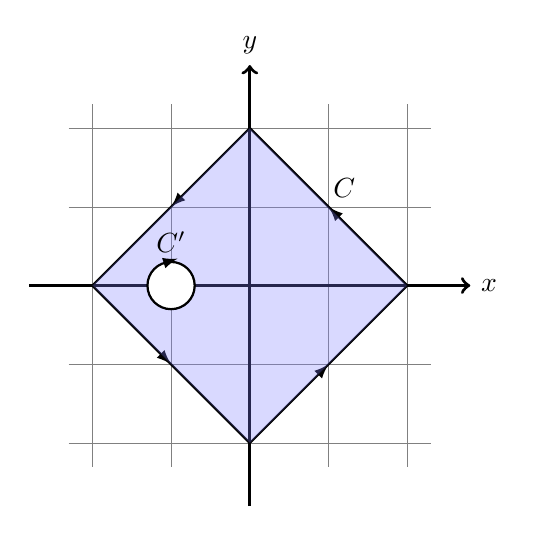
\begin{tikzpicture}

%	\usetikzlibrary{decorations,arrows}
%	\usetikzlibrary{decorations.markings}
	\draw[style=help lines,step=1cm] (-2.3,-2.3) grid (2.3,2.3);
	
	\draw[->,very thick] (-2.8,0) -- (2.8,0) node[right] {$x$};
	\draw[->,very thick] (0,-2.8) -- (0,2.8) node[above] {$y$};
	
	\tikzset{->-/.style=
		{decoration={markings,mark=at position #1 with 
				{\arrow{latex}}},postaction={decorate}}}
	\draw[thick,->-=0.5](2,0) -- (0,2);
	\draw[thick,->-=0.5](0,2) -- (-2,0);
	\draw[thick,->-=0.5](-2,0) -- (0,-2);
	\draw[thick,->-=0.5](0,-2) -- (2,0);
	
	\filldraw[fill= blue!50,opacity=0.3] (2,0) -- (0,2) -- (-2,0) -- (0,-2) -- cycle;
	\filldraw[fill= white,opacity=1] (-1,0) circle (0.3);
	
	\draw[thick, decoration={markings, mark=at position 0.3 
		with {\arrow{latex reversed}}}, postaction={decorate}] (-1,0) circle (0.3);
	
	\node[above] at (1.2,1){$C$};
	\node[above] at (-1,0.3){$C'$};
\end{tikzpicture}

\quad

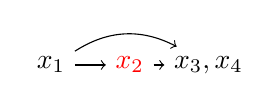
\begin{tikzpicture}
%	\usetikzlibrary{graphs}
	\graph {
		"$x_1$" -> "$x_2$"[red] -> "$x_3,x_4$";
		"$x_1$" ->[bend left] "$x_3,x_4$";
	};  
\end{tikzpicture}

\quad

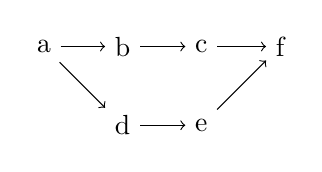
\begin{tikzpicture}
	\graph  {
		a -> {
			b -> c,
			d -> e 
		} -> f
	};
\end{tikzpicture}

\end{document}